\documentclass{beamer}
\mode<presentation>
\usepackage{amsmath}
\usepackage{amssymb}
\usepackage{algorithmic}
%\usepackage{advdate}
\usepackage{adjustbox}
\usepackage{subcaption}
\usepackage{enumitem}
\usepackage{multicol}
\usepackage{mathtools}
\usepackage{listings}
\usepackage{url}
\def\UrlBreaks{\do\/\do-}
% \usetheme{Boadilla}
% \usecolortheme{lily}
% \setbeamertemplate{footline}
% {
%   \leavevmode%
%   \hbox{%
%   \begin{beamercolorbox}[wd=\paperwidth,ht=2.25ex,dp=1ex,right]{author in head/foot}%
%     \insertframenumber{} / \inserttotalframenumber\hspace*{2ex} 
%   \end{beamercolorbox}}%
%   \vskip0pt%
% }
% \setbeamertemplate{navigation symbols}{}

% Theme settings
\usetheme{Singapore}     % Clean theme that works well with custom colors
\usecolortheme{orchid}   % Base purple color theme
\useinnertheme{circles}  % Circular bullets

% Define custom purple colors
\definecolor{deepPurple}{RGB}{81,40,136}
\definecolor{lightPurple}{RGB}{230,220,255}
\definecolor{mediumPurple}{RGB}{128,100,162}

% Apply custom colors
\setbeamercolor{structure}{fg=deepPurple}
\setbeamercolor{block title}{fg=white,bg=deepPurple}
\setbeamercolor{block body}{fg=black,bg=lightPurple}
\setbeamercolor{section in toc}{fg=deepPurple}
\setbeamercolor{alerted text}{fg=deepPurple}
\setbeamercolor{palette primary}{fg=white,bg=deepPurple}
\setbeamercolor{palette secondary}{fg=white,bg=mediumPurple}

% Remove navigation symbols
\setbeamertemplate{navigation symbols}{}

% Footer settings
\setbeamertemplate{footline}[frame number]

\providecommand{\nCr}[2]{\,^{#1}C_{#2}} % nCr
\providecommand{\nPr}[2]{\,^{#1}P_{#2}} % nPr
\providecommand{\mbf}{\mathbf}
\providecommand{\pr}[1]{\ensuremath{\Pr\left(#1\right)}}
\providecommand{\qfunc}[1]{\ensuremath{Q\left(#1\right)}}
\providecommand{\sbrak}[1]{\ensuremath{{}\left[#1\right]}}
\providecommand{\lsbrak}[1]{\ensuremath{{}\left[#1\right.}}
\providecommand{\rsbrak}[1]{\ensuremath{{}\left.#1\right]}}
\providecommand{\brak}[1]{\ensuremath{\left(#1\right)}}
\providecommand{\lbrak}[1]{\ensuremath{\left(#1\right.}}
\providecommand{\rbrak}[1]{\ensuremath{\left.#1\right)}}
\providecommand{\cbrak}[1]{\ensuremath{\left\{#1\right\}}}
\providecommand{\lcbrak}[1]{\ensuremath{\left\{#1\right.}}
\providecommand{\rcbrak}[1]{\ensuremath{\left.#1\right\}}}
\theoremstyle{remark}
\newtheorem{rem}{Remark}
\newcommand{\sgn}{\mathop{\mathrm{sgn}}}
\providecommand{\abs}[1]{\left\vert#1\right\vert}
\providecommand{\res}[1]{\Res\displaylimits_{#1}} 
\providecommand{\norm}[1]{\lVert#1\rVert}
\providecommand{\mtx}[1]{\mathbf{#1}}
\providecommand{\mean}[1]{E\left[ #1 \right]}
\providecommand{\fourier}{\overset{\mathcal{F}}{ \rightleftharpoons}}
%\providecommand{\hilbert}{\overset{\mathcal{H}}{ \rightleftharpoons}}
\providecommand{\system}{\overset{\mathcal{H}}{ \longleftrightarrow}}
	%\newcommand{\solution}[2]{\textbf{Solution:}{#1}}
%\newcommand{\solution}{\noindent \textbf{Solution: }}
\providecommand{\dec}[2]{\ensuremath{\overset{#1}{\underset{#2}{\gtrless}}}}
\newcommand{\myvec}[1]{\ensuremath{\begin{pmatrix}#1\end{pmatrix}}}
\let\vec\mathbf

\lstset{
%language=C,
frame=single, 
% breaklines=true,
columns=fullflexible
}

\numberwithin{equation}{section}

\title{Find the Point of Intersection of Two Lines}
\author{S A Aravind Eswar - EE24BTECH11053}

\date{\today} 
\begin{document}

\begin{frame}
\titlepage
\end{frame}

\section*{Outline}
\begin{frame}
\tableofcontents
\end{frame}

\section{Problem}
\begin{frame}
\frametitle{Problem Statement}
    Solve the following set of equations,
    \begin{align}
        5x - 3y = 11\\
        -10x + 6y = -22
    \end{align}
\end{frame}

%\subsection{Literature}
\section{Solution}

\subsection{Theoretical Solution}
\begin{frame}
    \frametitle{Theoretical Solution}
    By observing the equations, we can tell that they are a pair of co-incident lines.
    \begin{align}
        \frac{5}{-10} = \frac{-3}{6} = \frac{11}{-22} = -2
    \end{align}
    Thus there are infinite number of solutions to the given pair of equations.
\end{frame}

\subsection{Numerical Solution}
\begin{frame}[allowframebreaks]
    \frametitle{Method of solving}
    We can solve a given set of linear equation using LU decomposition.

    Let,
    \begin{align}
        a_1x_1+a_2x_2 + \dots + a_nx_n = a_0\\
        b_1x_1+b_2x_2 + \dots + b_nx_n = b_0\\
        \vdots\\
        p_1x_1+p_2x_2 + \dots + p_nx_n = p_0
    \end{align}
    Be a system of equations with $n$ variables and $n$ equations.

    Then we can write the Given system of equations as,
    \begin{align}
        A\vec{x} = \vec{b}
    \end{align}
    where,
    \begin{align}
        A &= \myvec{a_1 & a_2 & \dots & a_n\\b_1 & b_2 & \dots & b_n\\\vdots & \vdots & \vdots & \vdots\\p_1 & p_2 & \dots & p_n}\\
        \vec{b} &= \myvec{a_0\\b_0\\\vdots\\p_0}\\
    \end{align}
    \begin{align}
        \vec{x} &= \myvec{x_1\\x_2\\\vdots\\x_n}
    \end{align}
    We can decompose,
    \begin{align}
        A = LU
    \end{align}
    Where $L$ is a lower triangular matrix and $U$ is a upper triangular matrix.

    Now the equation can be written as,
    \begin{align}
        LU\vec{x} = \vec{b}
    \end{align}
    Writing $U\vec{x} = \vec{y}$
    \begin{align}
        L\vec{y} = \vec{b}
    \end{align}

    Using back Substitution Method we can solve for $\vec{y}$
    
    Now,
    \begin{align}
        U\vec{x} = \vec{y}
    \end{align}

    Using forward Substitution, we can compute $\vec{x}$
\end{frame}

\subsubsection{Gaussian Elimination}
\begin{frame}[allowframebreaks]
    \frametitle{Gaussian Elimination}
    One way to perform LU decomposition is using Gaussian Elimination.
    Gaussian Elimination can be written in the following way.

    For a matrix,

    \begin{align}
        A = \myvec{a_{11} & a_{12} & \dots & a_{1n}\\a_{21} & a_{22} & \dots & a_{2n}\\\vdots & \vdots & \vdots & \vdots\\a_{n1} & a_{n2} & \dots & a_{nn}}
    \end{align}

    Given that the diagonal elements aren't zero, we can reduce the first column as,

    \begin{align}
        R_i = R_i - \frac{a_{i1}}{a_{11}}R_1\\
        R_i = R_i - l_{i1}R_1
    \end{align}
    where $i>1$

    Similarly reduing other $n-2$ columns, $A$ is transformed into an upper triangular matrix $U$.

    In general, we can write it as,

    \begin{align}
        R_i = R_i - \frac{a_{ij}}{a_{jj}}R_1\\
        R_i = R_i - l_{ij}R_1
    \end{align}

    $L$ is given by,
    \begin{align}
        L = \myvec{1 & 0 & 0 & \dots & 0\\l_{21} & 1 & 0 & \dots & 0\\ l_{31} & l_{32} & 1 & \dots & 0\\
        \vdots & \vdots & \vdots & \vdots & \vdots\\l_{n1} & l_{n2} & l_{n3} & \dots & 1}
    \end{align}

    Where,

    \begin{align}
        l_{ij} = \frac{a_{ij}}{a_{ii}}
    \end{align}

    If the diagonal elements are zero, then we multiply $A$ with a permutation matrix
 $P$ and pivot it such that the diagonal elements become non-zero. 
\end{frame}

\begin{frame}
    \frametitle{Gaussian Elimination Algorithm}

    \begin{algorithmic}
        \FOR{$i$ in range($n$)}
            \FOR{$j$ in range($n-1$, $i$, $-1$)}
                \STATE $l_{ji} = A_{j,i}/A_{i,i}$
                \STATE $U_{j,:} = A_{j,:} - l_{ji}A_{i,:}$
                \STATE $L_{j,i} = l_{ji}$
            \ENDFOR
        \ENDFOR
    \end{algorithmic}
\end{frame}

\subsubsection{Doolittle's Algorithm}
\begin{frame}[allowframebreaks]
\frametitle{Doolittle's Algorithm}
    Doolittle's algorithm provides a more elegant and better method to perform LU decomposition.

    Doolittle's algorithm is given by,

    For $U$
    \begin{align}
        \forall &j\\
        i = 0 &\to U_{ij} = A_{ij}\\
        i > 0 &\to U_{ij} = A_{ij} - \sum_{k=0}^{i-1}L_{ik}U_{kj}
    \end{align}

    For $L$
    \begin{align}
        \forall &i\\
        j=0 &\to L_{ij} = \frac{A_{ij}}{U_{jj}}\\
        j>0 &\to L_{ij} = \frac{A_{ij} - \sum_{k=0}^{j-1}L_{ik}U_{kj}}{U_{jj}}
    \end{align}

    After performing LU decomposition, we get,
    \begin{align}
        A = LU
    \end{align}

    where,
    \begin{align}
        L = \myvec{1 & 0\\-2 & 1}\\
        U = \myvec{5 & -3\\0 & 0}
    \end{align}

\end{frame}

\begin{frame}[allowframebreaks]
    \frametitle{Doolittle Algorithm}
        \begin{algorithmic}
            \STATE $L$, $U  \gets n\times n$ zero arrays
            \FOR{$i$ in range($n$)}
                \FOR{$k$ in range($i,n$)}
                    \STATE $sum \gets 0$
                    \FOR{$j$ in range($i$)}
                        \STATE $sum \gets sum + L_{i,j} \, U_{j,k}$
                    \ENDFOR
                    \STATE $U_{i,k} \gets A_{i,k} - sum$
                \ENDFOR

                \FOR{$k$ in range($i$, $n$)}
                    \IF{$i=k$}
                        \STATE $L_{i,k} \gets 1$
                    \ELSE
                        \STATE $sum \gets 0$
                        \FOR{$j$ in range($i$)}
                            \STATE $sum \gets sum+L_{k,j}\,U_{j,i}$
                        \ENDFOR
                        \STATE $L_{k,i} \gets (A_{k,i} - sum) - U_{i,i}$
                    \ENDIF
                \ENDFOR
            \ENDFOR

        \end{algorithmic}
\end{frame}

\subsection{Plotting the curve}
\begin{frame}
\frametitle{Plotting the curve}
\begin{figure}[h]
    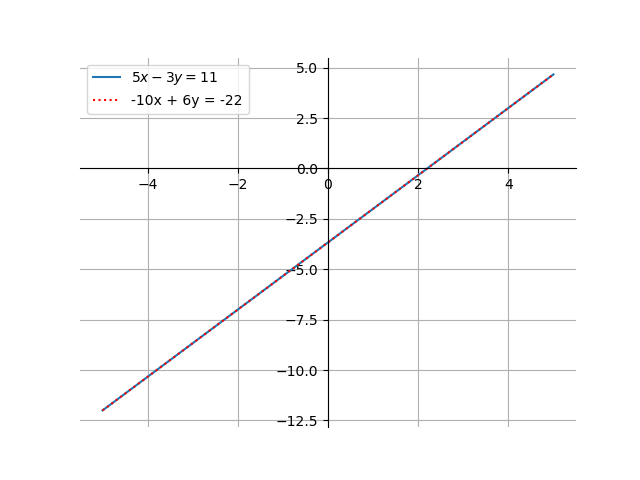
\includegraphics[scale=0.59]{../figs/fig1.png}
\centering
\end{figure}
\end{frame}

\end{document}
